\documentclass[xcolor=dvipsnames,serif,10pt]{beamer}

\usepackage{beamerthemesplit}
\usepackage{graphics}
\usepackage{graphicx}
\usepackage{hyperref}
\usepackage[normalem]{ulem}
%\usefonttheme{professionalfonts}
%\usepackage{times}
\usepackage{tikz}
\usepackage{amsmath}
\usepackage{verbatim}
\usetikzlibrary{arrows,shapes}
\usepackage{listings}


    \definecolor{listcomment}{rgb}{0.0,0.5,0.0}
    \definecolor{listkeyword}{rgb}{0.0,0.0,0.5}
    \definecolor{listnumbers}{gray}{0.65}
    \definecolor{listlightgray}{gray}{0.955}
    \definecolor{listwhite}{gray}{1.0}


\usetheme[secheader]{Boadilla}
\useoutertheme{miniframes}
\useinnertheme{circles}
\usecolortheme{myct}
\usepackage[latin1]{inputenc}


\newcommand\fontvi{\fontsize{6}{8}\selectfont}
\newcommand{\ColIndent}{\hspace{\labelwidth}\hspace{\labelsep}\hspace{\labelsep}\hspace{\labelsep}\hspace{\labelsep}}

%%%%%%%%%%%%%%%%%%%%%%%%%%%%%
%%  Title slide
%%%%%%%%%%%%%%%%%%%%%%%%%%%%%

\title[Time-Varying DMFFD]{Diffeomorphic directly manipulated free-form deformation
image registration via vector field flows}
\author[Tustison \& Avants]{%
  Nick Tustison\inst{1} \and
  Brian Avants\inst{2}
  }
\date[WBIR 2012]{}
\institute[PICSL]{%
  \inst{1} Department of Radiology and Medical Imaging\\
  University of Virginia
  \and
  \inst{2} Penn Image Computing and Science Laboratory\\
  University of Pensylvania
  }

%\pgfdeclaremask{fsu}{fsu_logo_ybkgrd}
%\pgfdeclareimage[width=1cm]{logo}{ants_logo}
%\logo{\vbox{\vskip0.1cm\hbox{\pgfuseimage{logo}}}}

\logo{
  
\includegraphics[height=0.8cm]{ants_logo.png}
  
\includegraphics[height=0.8cm]{itkLogo.jpg}
  }

\begin{document}

\tikzstyle{every picture}+=[remember picture]

\frame{\titlepage}

%%%%%%%%%%%%%%%%%%%%%%%%%%%%%
%%  Outline
%%%%%%%%%%%%%%%%%%%%%%%%%%%%%

\frame {
	\frametitle{Preliminaries}
	\begin{itemize}
		\item<1->My apologies to Reviewer 2,
		\item<2->Towards a generalization of the current work,
		\item<3->Focus on implementation (particularly the Insight Toolkit), and
		\item<4->Open source availability in ITK, ANTs, and/or Insight Journal.
	\end{itemize}
	}

%\begin{frame}
%\fontvi
%\begin{block}{Outline of talk - 22.5 minutes total per speaker}
%\begin{itemize}
%  \item opening - apologies to reviewer 2
%  \item history
%    \begin{itemize}
%      \fontvi
%      \item wrote \texttt{itkBSplineScatteredDataPointSetToImageFilter}
%      \item worked with Brian and Gang to develop ANTs
%      \item created a FFD-type algorithm (TIP 2009)
%      \item also created N4 and the point set registration algorithm
%      \item then came ITKv4 development (Brian will talk more about this later)
%    \end{itemize}
%  \item image registration algorithmic development
%    \begin{itemize}
%      \fontvi
%      \item wrote Diffeomorphic DMFFD (slides:  math, implementation)
%      \item wrote B-spline SyN (slides:  math, implementation)
%      \item overview of antsRegistration (slides:  summary of contributions, command line call)
%    \end{itemize}  
%  \item results
%    \begin{itemize}
%      \fontvi
%      \item Evaluation data description
%      \item \sout{LPBA40 study (slides:  results from paper)}
%      \item \sout{NIREP study (slides: overlap, timing, convergence)}
%    \end{itemize}  
%  \item closing  
%\end{itemize}
%\end{block}
%
%\end{frame}

%%%%%%%%%%%%%%%%%%%%%%%%%%%%%
%%  Background
%%%%%%%%%%%%%%%%%%%%%%%%%%%%%

%\begin{frame}{A little background\ldots}
%  \begin{center}
%  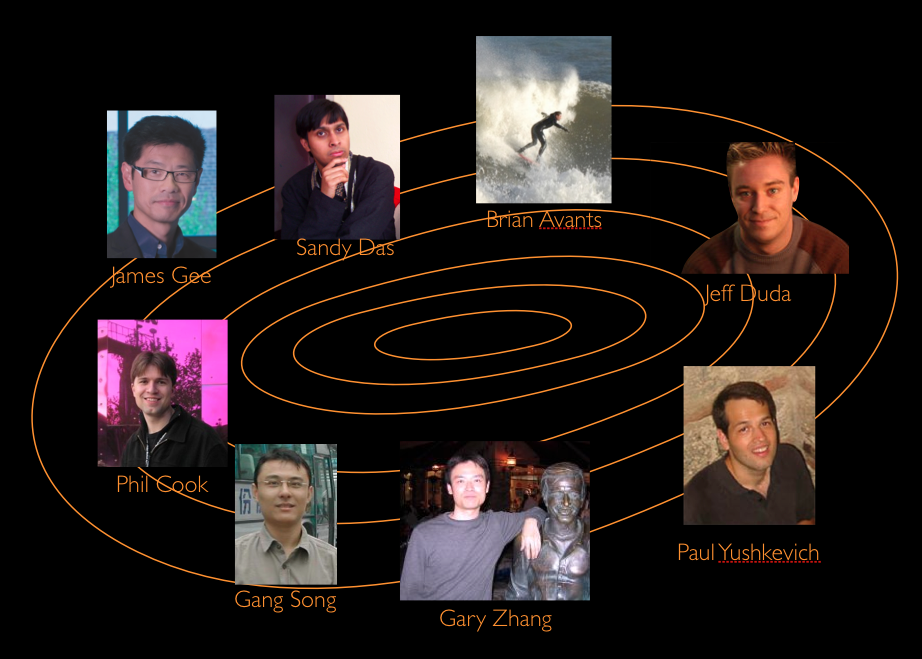
\includegraphics[height=6cm]{PICSL.png}
%  \end{center}
%\end{frame}

%%%%%%%%%%%%%%%%%%%%%%%%%%%%%
%%  background 2
%%%%%%%%%%%%%%%%%%%%%%%%%%%%%

\begin{frame}{http://sourceforge.net/projects/advants/}
  \begin{center}
  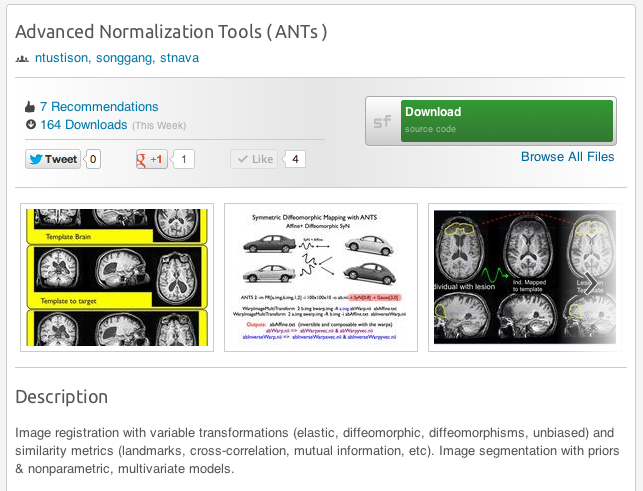
\includegraphics[height=6cm]{ANTSSourceforge.png}
  \end{center}
\end{frame}

%%%%%%%%%%%%%%%%%%%%%%%%%%%%%
%%  background 3
%%%%%%%%%%%%%%%%%%%%%%%%%%%%%

\begin{frame}{Basic ANTs registration}
  \begin{center}
    \begin{enumerate}
    \item Compute update field $u$.
    \item Smooth for fluid-like registration, i.e. $u \leftarrow K_{fluid} \star u$.
    \item Add to the total field, $s$, i.e. $s \leftarrow s + u$.
    \item Smooth for elastic-like registration, i.e. $s \leftarrow K_{elastic} \star s$.
    \end{enumerate}
  \end{center}

Possible options for $K$:
  \begin{center}
    \begin{itemize}
    \item Gaussian smoothing or
    \item B-spline smoothing.
    \end{itemize}
  \end{center}
\end{frame}

%%%%%%%%%%%%%%%%%%%%%%%%%%%%%
%%  FFD vs. DMFFD math
%%%%%%%%%%%%%%%%%%%%%%%%%%%%%

%\begin{equation*}
%\vec{a}_p = \vec{a}_o+\frac{{}^bd^2}{dt^2}\vec{r} +
%        \tikz[baseline]{
%            \node[fill=blue!20,anchor=base] (t1)
%            {$ 2\vec{\omega}_{ib}\times\frac{{}^bd}{dt}\vec{r}$};
%        } +
%        \tikz[baseline]{
%            \node[fill=red!20, ellipse,anchor=base] (t2)
%            {$\vec{\alpha}_{ib}\times\vec{r}$};
%        } +
%        \tikz[baseline]{
%            \node[fill=green!20,anchor=base] (t3)
%            {$\vec{\omega}_{ib}\times(\vec{\omega}_{ib}\times\vec{r})$};
%        }
%\end{equation*}



\begin{frame}
\frametitle{Directly Manipulated Free Form Deformation Image Registration}
\begin{align*}
\mathcal{T} = \sum_{i_1=1}^{N_1}\ldots\sum_{i_d=1}^{N_d} \phi_{i_1,\ldots,i_d} \prod_{j=1}^d B_{i_j}(x_j) \nonumber
\end{align*}

\begin{itemize}
\item FFD
\begin{equation*}
\tikz[baseline]{
  \node[fill=blue!20,anchor=base,rounded corners, inner sep=4pt, inner ysep=4pt] (t1)
  {$\delta \phi_{i_1,\ldots,i_d} \propto \sum_{c=1}^{N_\Omega} \left( \frac{\partial \Pi}{\partial \mathcal{T}}\right)_c\prod_{j=1}^d B_{i_j}(x^c_j)$};
}  
\end{equation*}
\end{itemize}

\begin{itemize}
\item DMFFD
\begin{equation*}
\tikz[baseline]{
  \node[fill=green!20,anchor=base, rounded corners, inner sep=4pt, inner ysep=4pt] (t2)
{$\delta \phi_{i_1,\ldots,i_d} \propto \sum_{c=1}^{N_\Omega} \left( \frac{\partial \Pi}{\partial \mathcal{T}}\right)_c \frac{\prod_{j=1}^d B_{i_j}(x^c_j) \prod_{j=1}^d B_{i_j}^2 (x_j^c)}{\sum_{k_1=1}^{N_1}\ldots\sum_{k_d=1}^{N_d} \prod_{j=1}^d B_{k_j}^2 (x_j^c)}$};
}
\end{equation*}
\end{itemize}

\end{frame}

%%%%%%%%%%%%%%%%%%%%%%%%%%%%%
%%  Applications of b-spline fitting
%%%%%%%%%%%%%%%%%%%%%%%%%%%%%

\begin{frame}{B-spline fitting applications}

\tikzstyle{mybox} = [draw=black, fill=beamer@blendedblue!40, thick,
    rectangle, rounded corners, inner sep=10pt, inner ysep=10pt]
\tikzstyle{mybox2} = [draw=black, fill=beamer@blendedblue!40, thick,
    rectangle, rounded corners, inner sep=2pt, inner ysep=5pt, 
    minimum height=4cm]
\tikzstyle{fancytitle} =[fill=beamer@blendedblue, text=white, rectangle]
\tikzstyle{line} = [-latex',very thick,beamer@blendedblue]


\begin{center}
\begin{tikzpicture}
\node [mybox] (bspline){%
  \centering
  \texttt{itk::BSplineScatteredDataPointSetToImageFilter}
};
\end{tikzpicture}%
\end{center}
\vspace{5mm}


\begin{center}
\begin{tikzpicture}[node distance = 3cm]

\node [mybox2](DMFFD) {%  
  \begin{tabular}{c}
  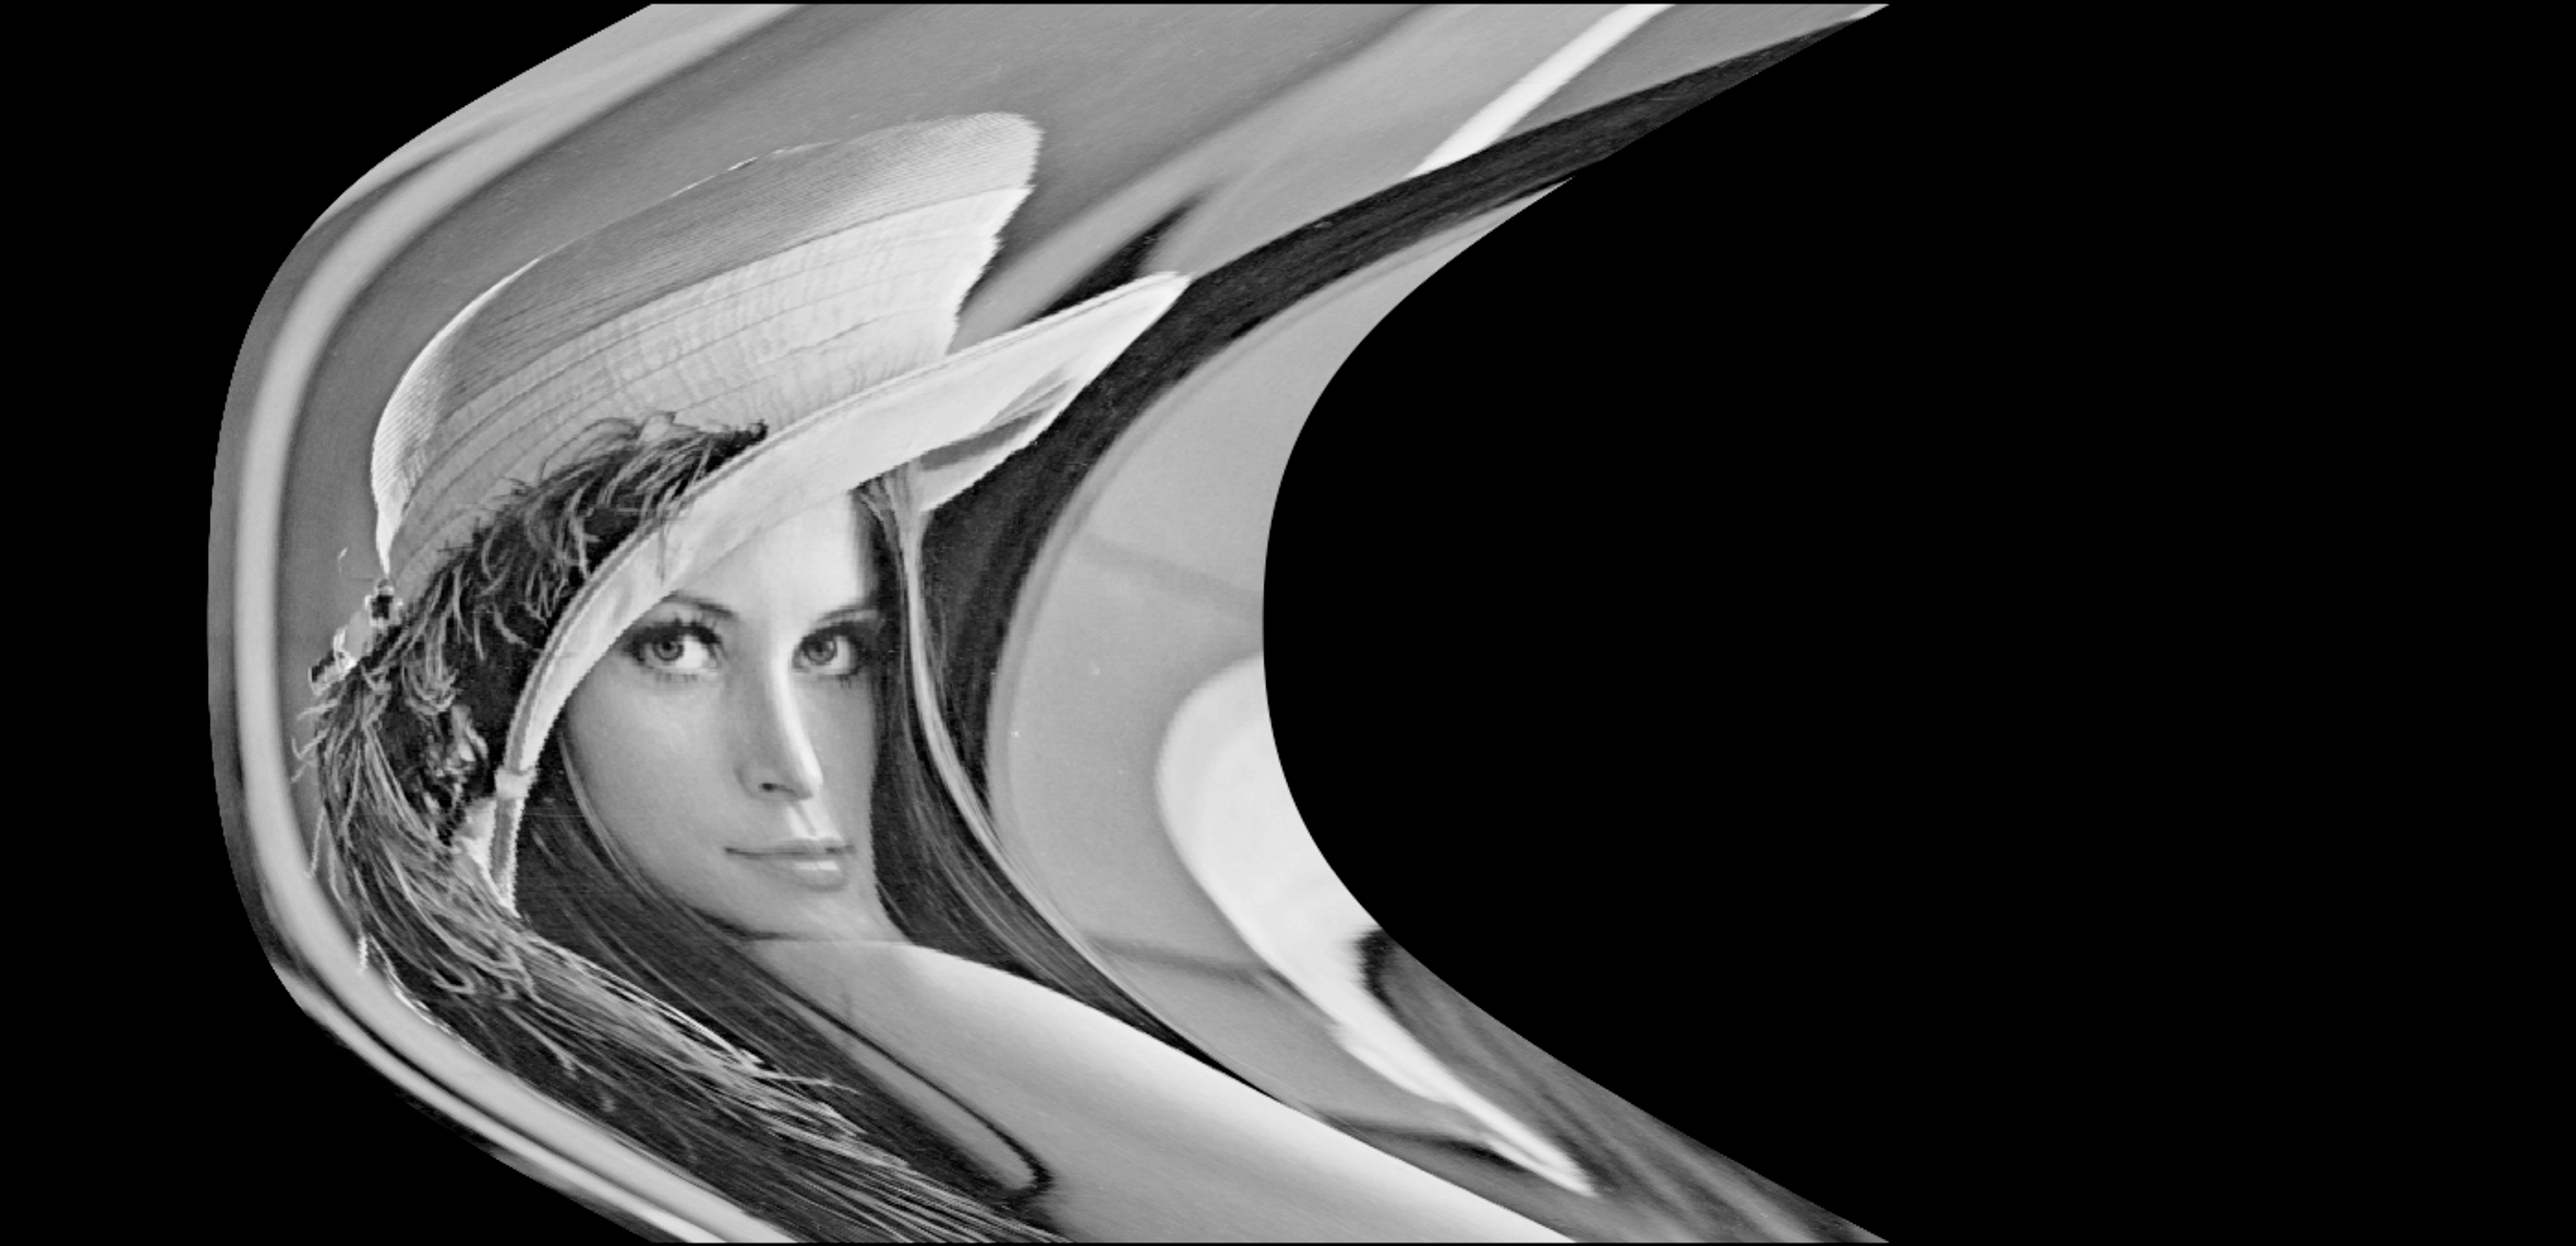
\includegraphics[height=1cm]{ffd.pdf} \\
  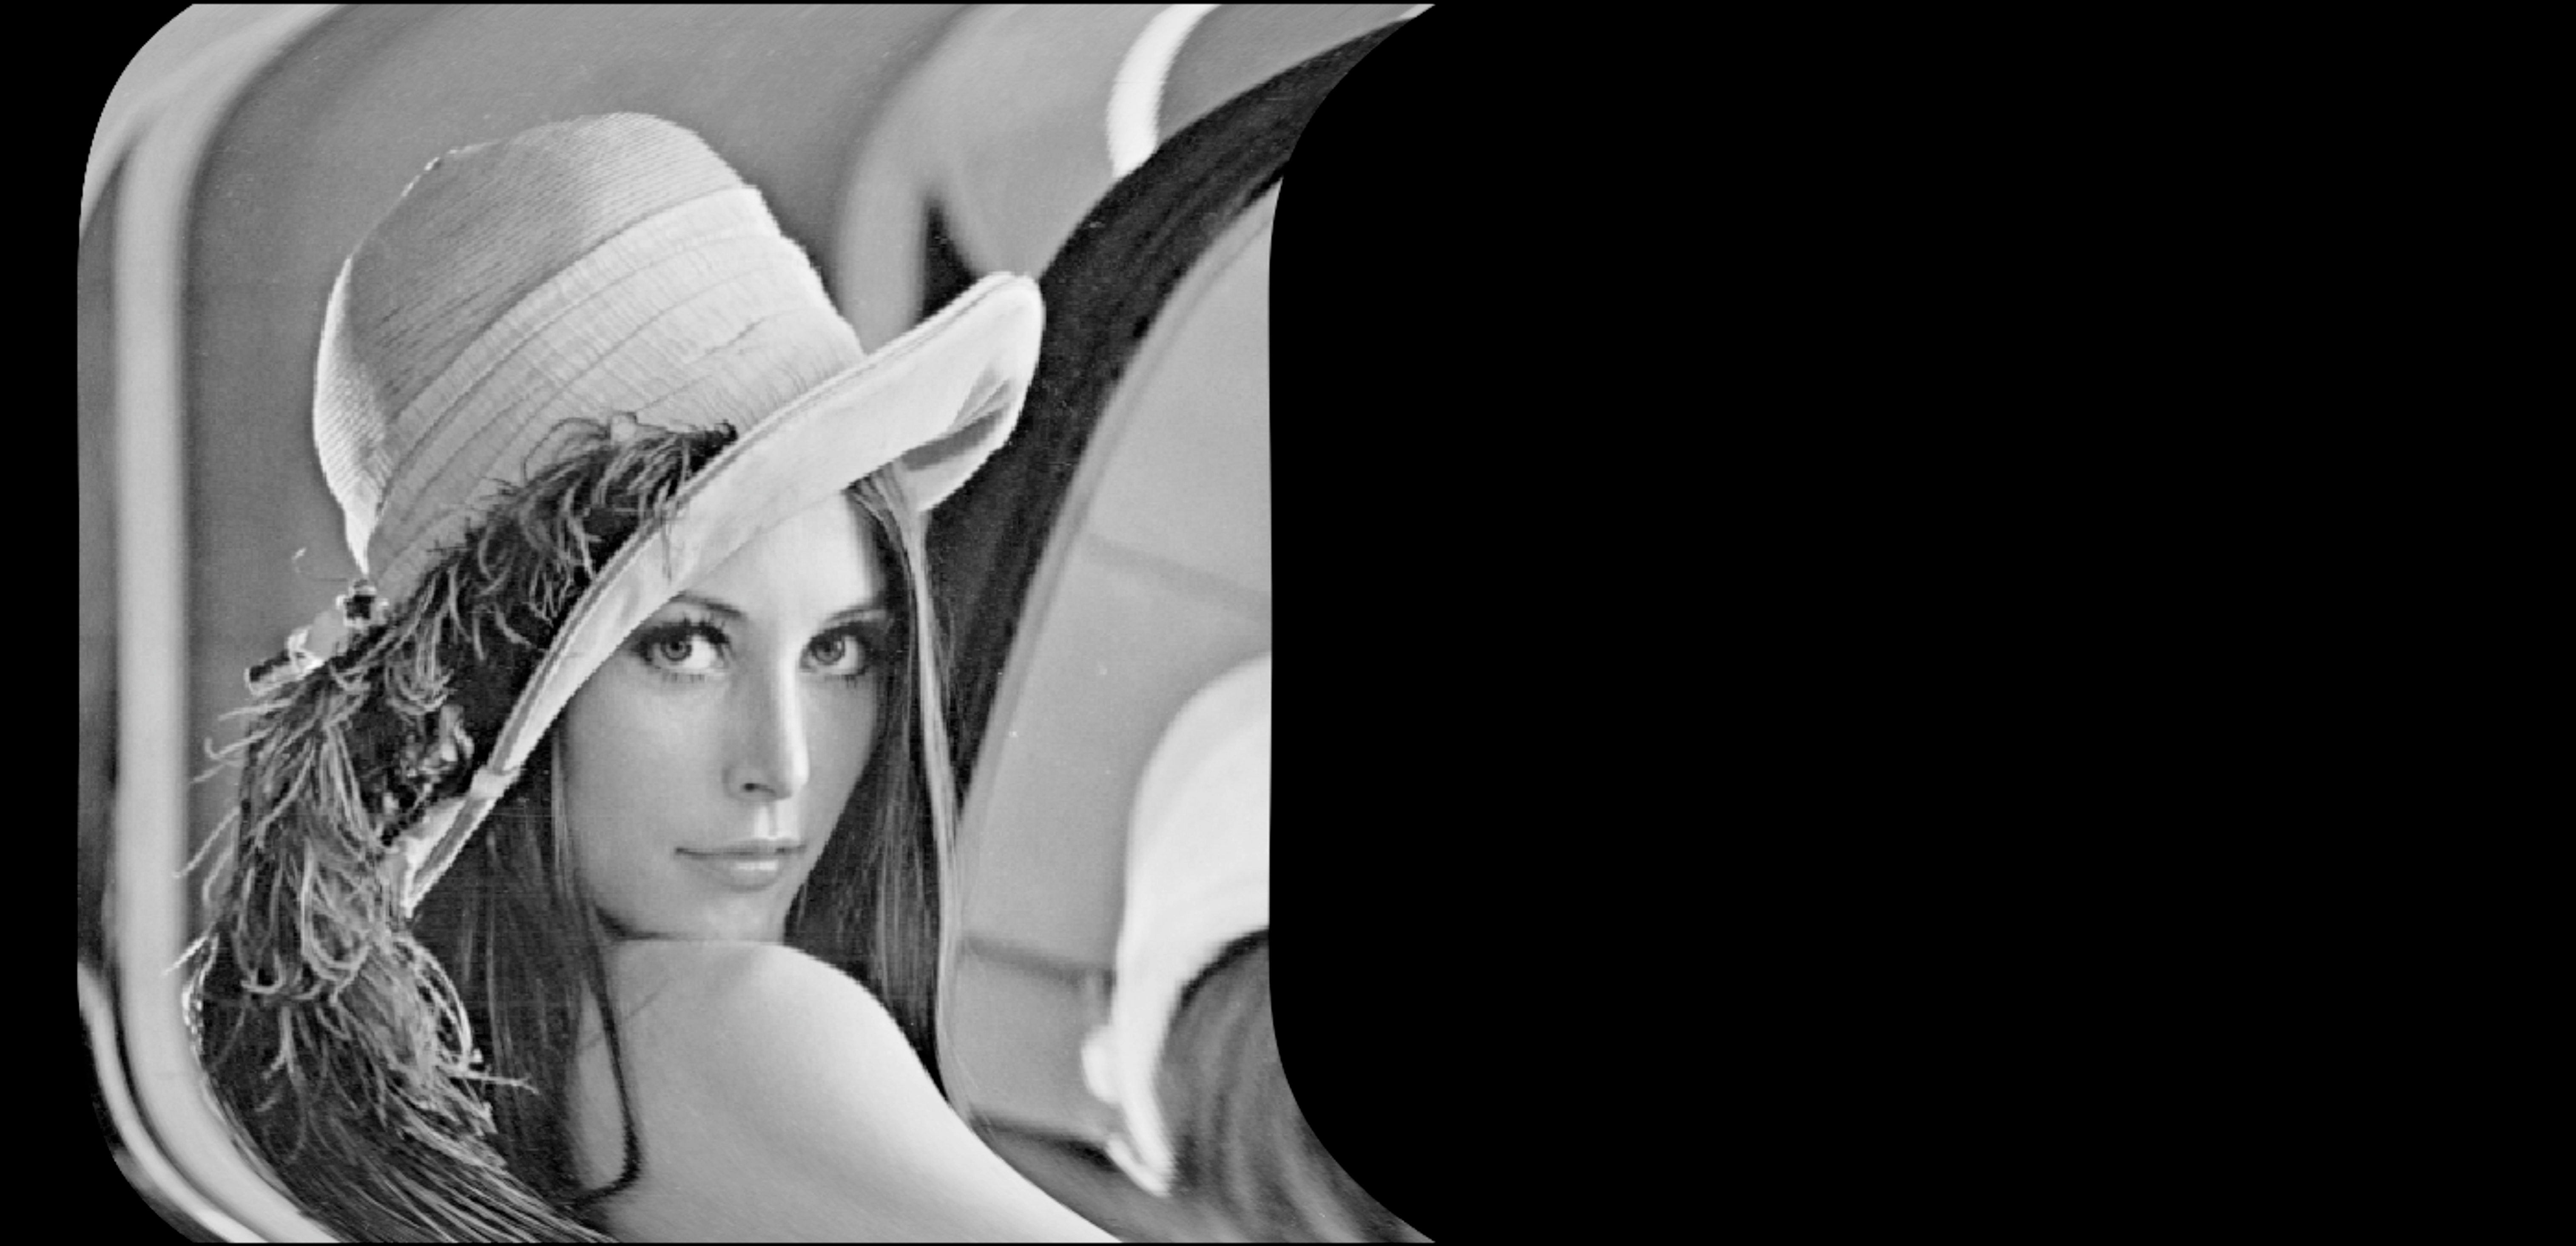
\includegraphics[height=1cm]{dmffd.pdf} \\
  \scriptsize{IEEE TIP 2009}
  \end{tabular}
  };
\node[fancytitle](DMFFDtitle) at (DMFFD.north) {\scriptsize Image reg.};

\node [mybox2, right of=DMFFD](N4) {
  \centering
  \begin{tabular}{c}
  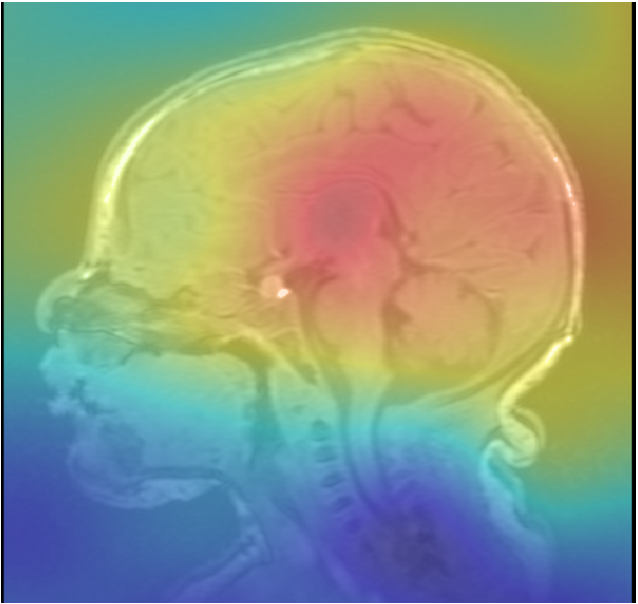
\includegraphics[height=2cm]{bias.pdf} \\
  \scriptsize{IEEE TMI 2010}
  \end{tabular}
  };
\node[fancytitle](N4title) at (N4.north) {\scriptsize Bias correction};

\node [mybox2, right of= N4](PSR) {%
  \centering
  \begin{tabular}{c}
  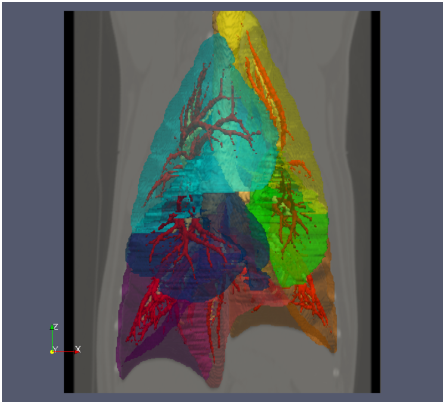
\includegraphics[height=2cm]{pointsetlungs.pdf} \\
  \scriptsize{IEEE TMI 2011}\\
  \vspace{-4mm}
  \scriptsize{JMRI 2010}\\
  \end{tabular}
  };
\node[fancytitle](PSRtitle) at (PSR.north) {\scriptsize Point set reg.};

\node [mybox2, dashed, right of=PSR](SyN) {
  \centering
  \begin{tabular}{c}
  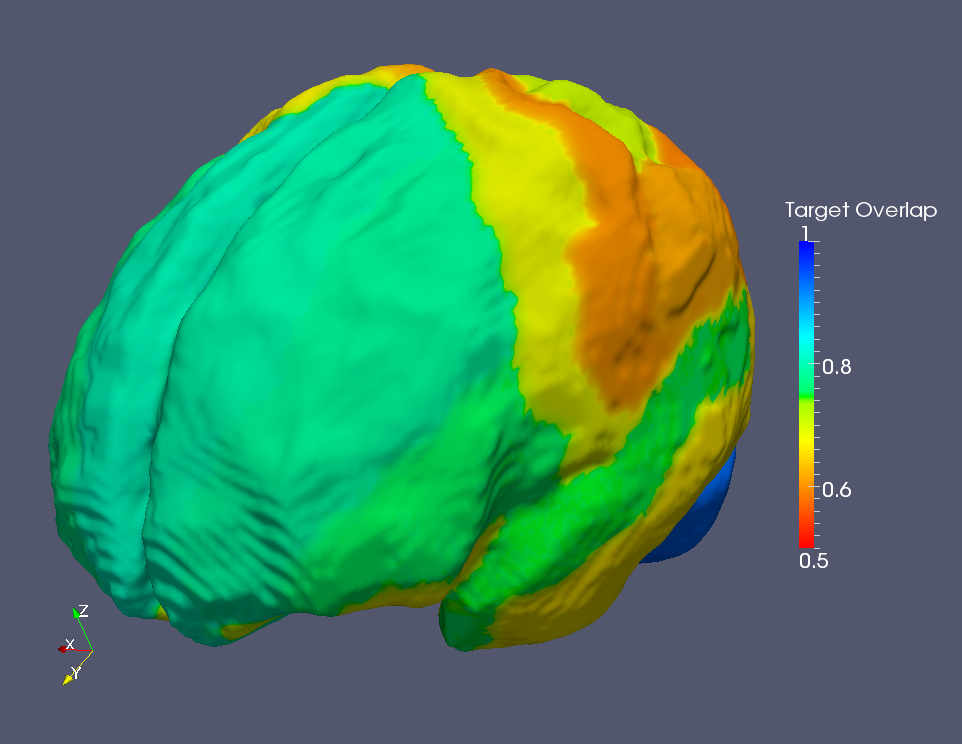
\includegraphics[height=1.75cm]{../Figures/leftHemisphere.png} \\
  \scriptsize{WBIR 2012}\\
  \end{tabular}
  };
\node[fancytitle](SyNtitle) at (SyN.north) {\scriptsize Diff. reg.};

\end{tikzpicture}

\begin{tikzpicture}
  \tikz[overlay]\path[line] (bspline.south) edge [out= 230, in= 90] (DMFFDtitle.north);
  \tikz[overlay]\path[line] (bspline.south) edge [out= 270, in= 90] (N4title.north);
  \tikz[overlay]\path[line] (bspline.south) edge [out= 270, in= 90] (PSRtitle.north);
  \tikz[overlay]\path[line] (bspline.south) edge [out= 310, in= 90] (SyNtitle.north);
\end{tikzpicture}

\end{center}

\end{frame}


%%%%%%%%%%%%%%%%%%%%%%%%%%%%%
%%  Time-varying DMFFD math
%%%%%%%%%%%%%%%%%%%%%%%%%%%%%

\begin{frame}{Time-Varying DMFFD}
Similarly, for the time-varying velocity field case we propose the following preconditioned gradient,
$\delta v_{i_1,\ldots,i_d,i_t}$, given the similarity metric, $\Pi$,%
\begin{align}
  \delta v_{i_1,\ldots,i_d,i_t} \propto& \left( \sum_{c=1}^{N_{\Omega} \times N_t} \left( \frac{\partial \Pi}{\partial \mathbf{x}} \right)_c B_{i_t}(t^c)\prod_{j=1}^d B_{i_j}(x_j^c)  \right. \nonumber \\
  &\cdot \left. \frac{B_{i_t}^2(t^c) \prod_{j=1}^d B_{i_j}^2 (x_j^c)} 
  {\sum_{k_1=1}^{r+1}\ldots\sum_{k_d=1}^{r+1} \sum_{k_t=1}^{r+1} B_{k_t}^2(t^c) 
  \prod_{j=1}^d B_{k_j}^2 (x_j^c)} \right) \nonumber 
\end{align}

\end{frame}



%%%%%%%%%%%%%%%%%%%%%%%%%%%%%
%%  ITK implementation
%%%%%%%%%%%%%%%%%%%%%%%%%%%%%

\begin{frame}{Implementation}

\begin{block}{ITK code}
\begin{itemize}
  \fontsize{8}{9}\selectfont
  \item \texttt{itk::BSplineScatteredDataPointSetToImageFilter}
  \item \texttt{itk::DisplacementFieldToBSplineImageFilter}
  \item \texttt{itk::BSplineSmoothingOnUpdateDisplacementFieldTransform} 
  \item \texttt{itk::BSplineSmoothingOnUpdateDisplacementFieldTransformParametersAdaptor} 
  \item \texttt{itk::TimeVaryingVelocityFieldIntegrationImageFilter} 
  \item \texttt{itk::TimeVaryingBSplineVelocityFieldTransform} 
  \item \texttt{itk::TimeVaryingBSplineVelocityFieldImageRegistrationMethod}
  \item \texttt{itk::TimeVaryingBSplineVelocityFieldTransformParametersAdaptor}
  \item \texttt{itk::TimeVaryingBSplineVelocityFieldIntegrationImageFilter}$^*$ 
  \item \texttt{itk::BSplineSyNImageRegistrationMethod}
\end{itemize}
\end{block}

\begin{block}{ANTs code}
\begin{itemize}
  \fontsize{8}{9}\selectfont
  \item \texttt{antsRegistration} 
  \item \texttt{itk::antsRegistrationHelper} 
\end{itemize}
\end{block}

\end{frame}

%%%%%%%%%%%%%%%%%%%%%%%%%%%%%
%%  antsRegistration
%%%%%%%%%%%%%%%%%%%%%%%%%%%%%

\lstset{frame = htb,
        framerule = 0.25pt,
        float,
        fontadjust,
        backgroundcolor={\color{listlightgray}},
        basicstyle = {\ttfamily\tiny},
        keywordstyle = {\ttfamily\color{listkeyword}\textbf},
        identifierstyle = {\ttfamily},
        commentstyle = {\ttfamily\color{listcomment}\textit},
        stringstyle = {\ttfamily},
        showstringspaces = false,
        showtabs = false
        numbers = none,
        numbersep = 6pt,
        numberstyle={\ttfamily\color{listnumbers}},
        tabsize = 2,
        language=bash,
        floatplacement=!h,
%        caption={Representative script used for the LPBA40 evaluation.},
        captionpos=b,
        label=listing:script
        }

\begin{frame}[fragile]
\frametitle{antsRegistration}
\begin{lstlisting}
COMMAND: 
     antsRegistration

OPTIONS: 
     -d, --dimensionality 2/3
     -o, --output outputTransformPrefix
                  [outputTransformPrefix,<outputWarpedImage>,<outputInverseWarpedImage>]
     -m, --metric CC[fixedImage,movingImage,metricWeight,radius,...]
                  MI[fixedImage,movingImage,metricWeight,numberOfBins,...]
                  Mattes[fixedImage,movingImage,metricWeight,numberOfBins,...]
                  MeanSquares[fixedImage,movingImage,metricWeight,radius=NA,...]
                  Demons[fixedImage,movingImage,metricWeight,radius=NA,...]
                  GC[fixedImage,movingImage,metricWeight,radius=NA,...]
     -t, --transform Rigid[gradientStep]
                     Affine[gradientStep]
                     CompositeAffine[gradientStep]
                     Similarity[gradientStep]
                     Translation[gradientStep]
                     BSpline[gradientStep,meshSizeAtBaseLevel]
                     GaussianDisplacementField[gradientStep,updateFieldVariance,totalFieldVariance]
                     BSplineDisplacementField[gradientStep,updateFieldMeshSize,totalFieldMeshSize,...]
                     TimeVaryingVelocityField[gradientStep,numberOfTimeIndices,updateFieldVariance,...]
                     TimeVaryingBSplineVelocityField[gradientStep,velocityFieldMeshSize,...]
                     SyN[gradientStep,updateFieldVarianceInVoxelSpace,totalFieldVarianceInVoxelSpace]
                     BSplineSyN[gradientStep,updateFieldMeshSize,totalFieldMeshSize,<splineOrder=3>]
     -c, --convergence MxNxO
                       [MxNxO,<convergenceThreshold=1e-6>,<convergenceWindowSize=10>]
     -s, --smoothing-sigmas MxNxO...
     -f, --shrink-factors MxNxO...
     -u, --use-histogram-matching 
     -l, --use-estimate-learning-rate-once 
     -w, --winsorize-image-intensities [lowerQuantile,upperQuantile]
     -x, --masks [fixedImageMask,movingImageMask]
     -h 
     --help 

\end{lstlisting}                 
\end{frame}

%%%%%%%%%%%%%%%%%%%%%%%%%%%%%
%%  Data description
%%%%%%%%%%%%%%%%%%%%%%%%%%%%%

\begin{frame}{Evaluation data}
     \begin{columns}[t] % contents are top      vertically aligned
     \begin{column}[t]{4cm} % each column can also be its own environment
       \begin{tabular}{c}
       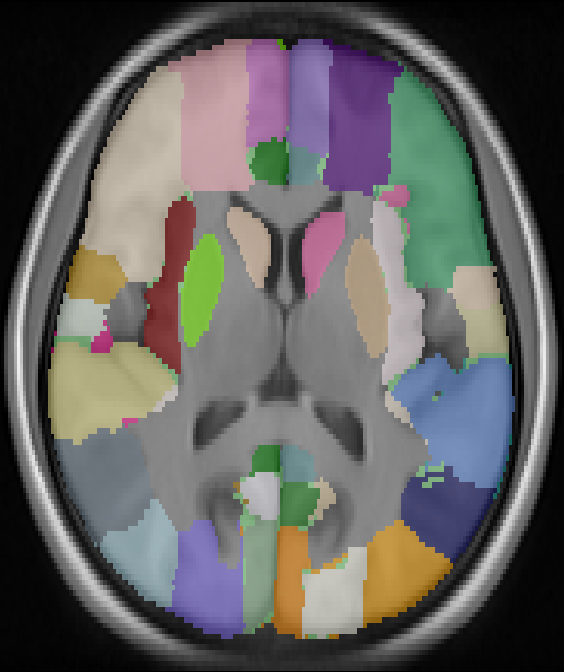
\includegraphics[height=6cm]{LPBA40Labels.png} \\
       LPBA40 
%       (ANTs template + STAPLE)
       \end{tabular}
     \end{column}
     \begin{column}[t]{5cm} % alternative top-align that's better for graphics
       \begin{tabular}{c}
       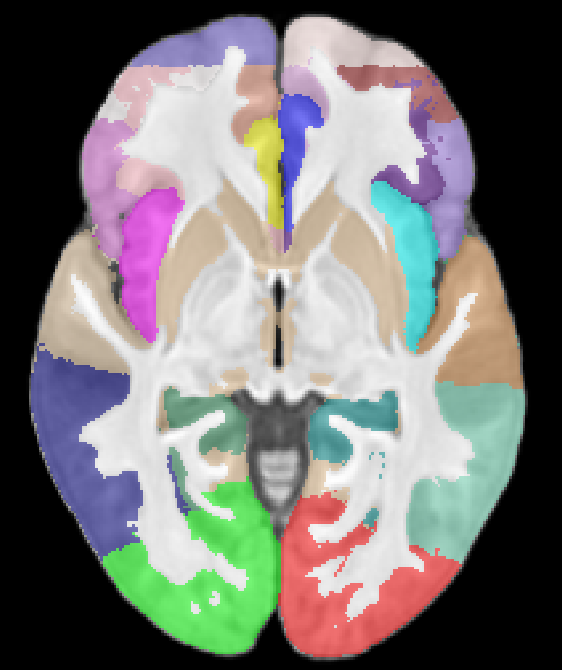
\includegraphics[height=6cm]{NIREPLabels.png} \\
       NIREP 
%       (ANTs template + STAPLE) 
       \end{tabular}
     \end{column}
     \end{columns}
\end{frame}

%%%%%%%%%%%%%%%%%%%%%%%%%%%%%
%%  LPBA40 evaluation command line calls
%%%%%%%%%%%%%%%%%%%%%%%%%%%%%

\lstset{frame = htb,
        framerule = 0.25pt,
        float,
        fontadjust,
        backgroundcolor={\color{listlightgray}},
        basicstyle = {\ttfamily\tiny},
        keywordstyle = {\ttfamily\color{listkeyword}\textbf},
        identifierstyle = {\ttfamily},
        commentstyle = {\ttfamily\color{listcomment}\textit},
        stringstyle = {\ttfamily},
        showstringspaces = false,
        showtabs = false
        numbers = none,
        numbersep = 6pt,
        numberstyle={\ttfamily\color{listnumbers}},
        tabsize = 2,
        language=bash,
        floatplacement=!h,
%        caption={Representative script used for the LPBA40 evaluation.},
        captionpos=b,
        label=listing:script
        }

\begin{frame}[fragile]
\frametitle{Command line calls for LPBA40 evaluation}
\begin{lstlisting}
# Register the moving LPBA subject to the fixed LPBA subject.

antsRegistration --dimensionality 3 \
                 --output ${prefix} \
                 --use-histogram-matching 1 \
                 --transform Affine[0.5] \                # affine stage
                 --metric Demons[${fixed_n4},${moving_n4},1,0,Regular,0.01] \ 
                 --iterations 100x100x100 \
                 --smoothing-sigmas 4.0x3.0x2.0 \
                 --shrink-factors 4x3x2 \
                 --transform tvdmffd[0.75,24x24x12x1,4] \ # tv dmffd stage
                 --metric CC[${fixed_n4},${moving_n4},1,4] \ 
                 --iterations 40x50x2 \
                 --smoothing-sigmas 1.0x0.5x0.0 \
                 --shrink-factors 3x2x1

# Apply the resulting transforms (affine + tvdmffd) to the moving labels.
                   
antsApplyTransforms --dimensionality 3 \
                    --input ${moving_labels} \
                    --reference-image ${fixed_n4} \
                    --output ${moving_warped_labels} \
                    --interpolation NearestNeighbor \
                    --transform ${prefix}1Warp.nii.gz \
                    --transform ${prefix}0Affine.mat \
                    --default-value 0
\end{lstlisting}                 
\end{frame}

%%%%%%%%%%%%%%%%%%%%%%%%%%%%%
%%  LPBA40 total overlap results
%%%%%%%%%%%%%%%%%%%%%%%%%%%%%

\begin{frame}{LPBA40 regional target overlap}

\setlength{\tabcolsep}{4pt}

\fontsize{5}{6}\selectfont

\begin{columns}[totalwidth=0.7\textwidth,t]
\ColIndent
\begin{column}[t]{5cm}
\begin{tabular}{lc}
{\bf Region} & {\bf Overlap} \\
\hline
L superior frontal gyrus & 0.802 \\
R superior frontal gyrus & 0.810 \\
L middle frontal gyrus & 0.790 \\
R middle frontal gyrus & 0.778 \\
L inferior frontal gyrus & 0.753 \\
R inferior frontal gyrus & 0.728 \\
L precentral gyrus & 0.687 \\
R precentral gyrus & 0.674 \\
L middle orbitofrontal gyrus & 0.687 \\
R middle orbitofrontal gyrus & 0.671 \\
L lateral orbitofrontal gyrus & 0.669 \\
R lateral orbitofrontal gyrus & 0.607 \\
L gyrus rectus & 0.654 \\
R gyrus rectus & 0.652 \\
L postcentral gyrus & 0.604 \\
R postcentral gyrus & 0.620 \\
L superior parietal gyrus & 0.709 \\
R superior parietal gyrus & 0.701 \\
L supramarginal gyrus & 0.619 \\
R supramarginal gyrus & 0.623 \\
L angular gyrus & 0.594 \\
R angular gyrus & 0.620 \\
L precuneus & 0.668 \\
R precuneus & 0.659 \\
L superior occipital gyrus & 0.548 \\
R superior occipital gyrus & 0.561 \\
L middle occipital gyrus & 0.671 \\
R middle occipital gyrus & 0.696 \\
\hline
\end{tabular}
\end{column}
\begin{column}[t]{5cm}
\begin{tabular}{lc}
{\bf Region} & {\bf Overlap} \\
\hline
L inferior occipital gyrus & 0.621 \\
R inferior occipital gyrus & 0.637 \\
L cuneus & 0.622 \\
R cuneus & 0.624 \\
L superior temporal gyrus & 0.750 \\
R superior temporal gyrus & 0.737 \\
L middle temporal gyrus & 0.660 \\
R middle temporal gyrus & 0.644 \\
L inferior temporal gyrus & 0.662 \\
R inferior temporal gyrus & 0.674 \\
L parahippocampal gyrus & 0.711 \\
R parahippocampal gyrus & 0.707 \\
L lingual gyrus & 0.694 \\
R lingual gyrus & 0.681 \\
L fusiform gyrus & 0.703 \\
R fusiform gyrus & 0.719 \\
L insular cortex & 0.812 \\
R insular cortex & 0.768 \\
L cingulate gyrus & 0.691 \\
R cingulate gyrus & 0.676 \\
L caudate & 0.704 \\
R caudate & 0.717 \\
L putamen & 0.773 \\
R putamen & 0.761 \\
L hippocampus & 0.753 \\
R hippocampus & 0.742 \\
cerebellum & 0.935 \\
brainstem & 0.899 \\
\hline
\end{tabular}
\end{column}
\end{columns}

\end{frame}

%%%%%%%%%%%%%%%%%%%%%%%%%%%%%
%%  LPBA40 3D Results
%%%%%%%%%%%%%%%%%%%%%%%%%%%%%

\begin{frame}{LPBA40 results (cf Klein, NeuroImage 2009)}


\begin{center}
\begin{tabular}{cc}
  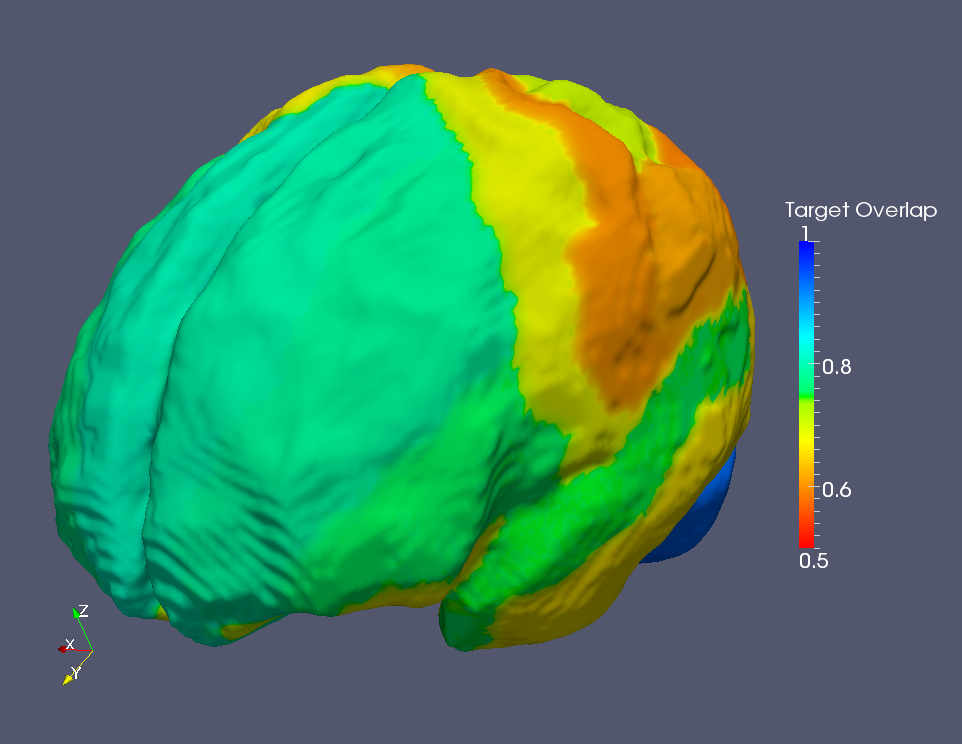
\includegraphics[width=55mm]{../Figures/leftHemisphere.png} &
  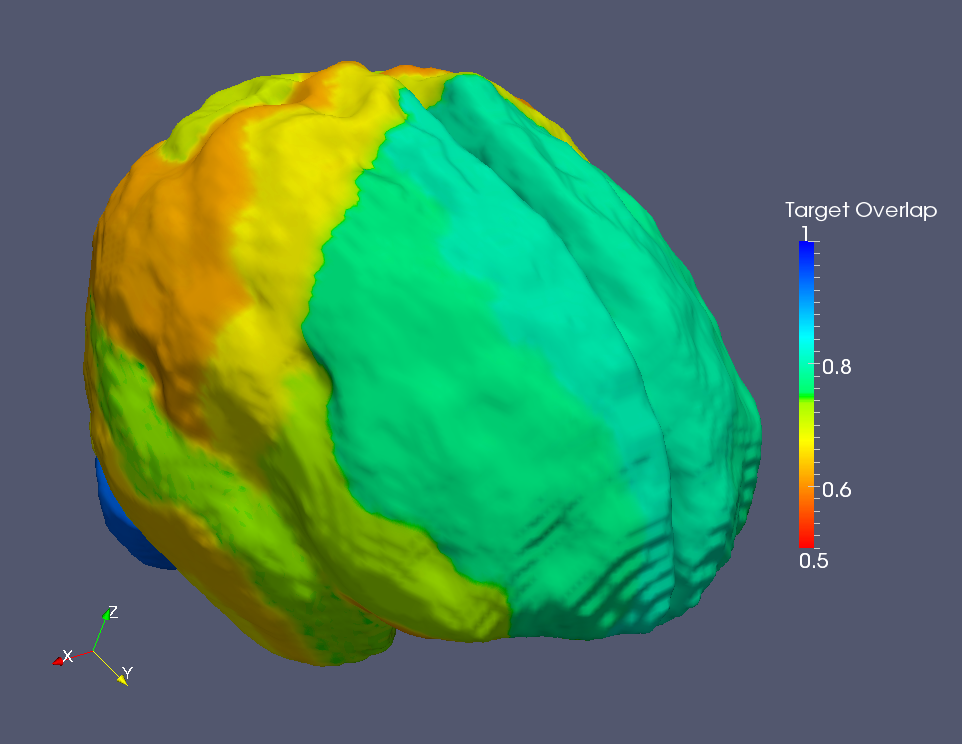
\includegraphics[width=55mm]{../Figures/rightHemisphere.png}
\end{tabular}
\end{center}

\end{frame}

%%%%%%%%%%%%%%%%%%%%%%%%%%%%%
%%  NIREP Results (label overlap)
%%%%%%%%%%%%%%%%%%%%%%%%%%%%%

\begin{frame}{SyN NIREP overlap results}

\begin{center}
\vspace*{-16mm}
\begin{tabular}{c}
  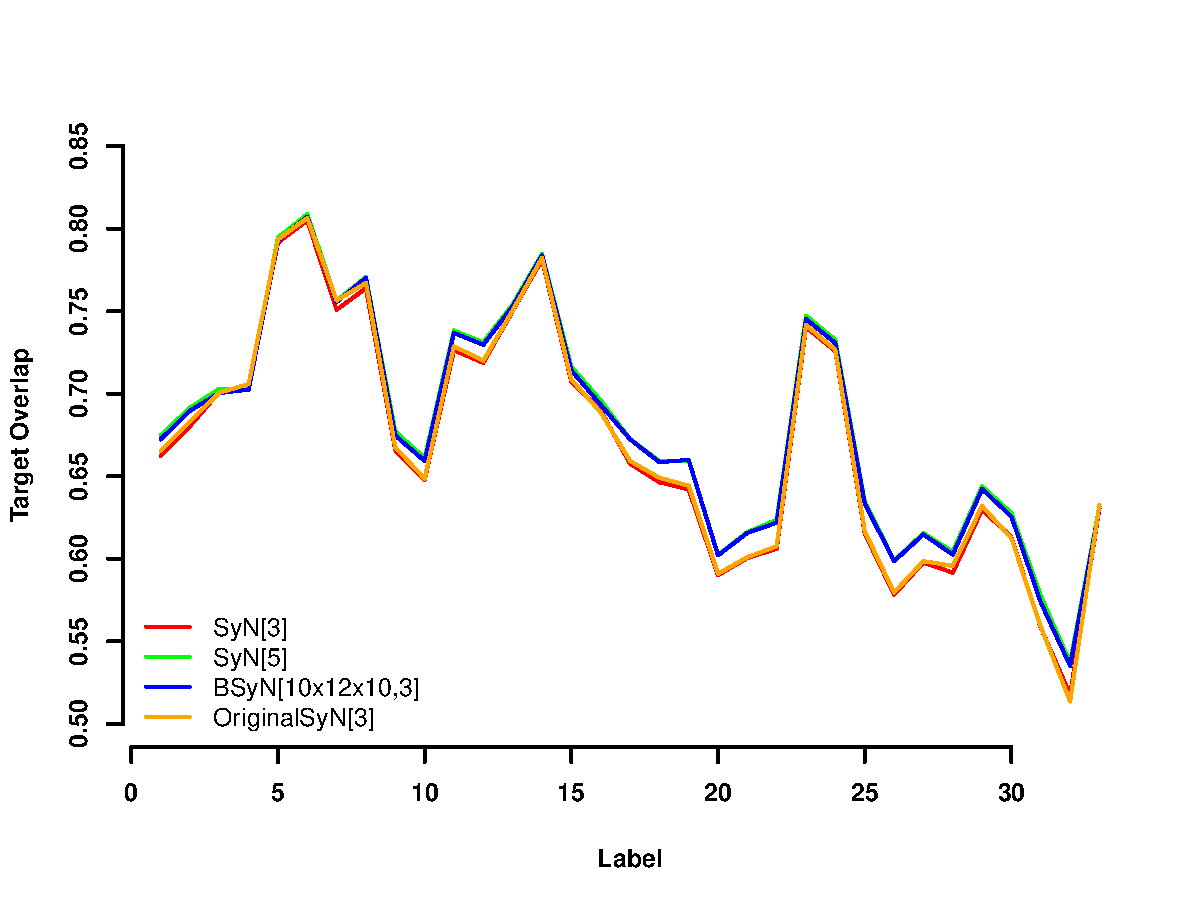
\includegraphics[width=120mm]{../WBIRStudy/SyNLabelOverlapNIREP.pdf}
\end{tabular}
\end{center}

\end{frame}

%%%%%%%%%%%%%%%%%%%%%%%%%%%%%
%%  NIREP Performance (convergence and metric evolution)
%%%%%%%%%%%%%%%%%%%%%%%%%%%%%

\begin{frame}{SyN NIREP performance}

\begin{center}
\vspace*{-10mm}
\begin{tabular}{cc}
  \hspace{-5mm}
  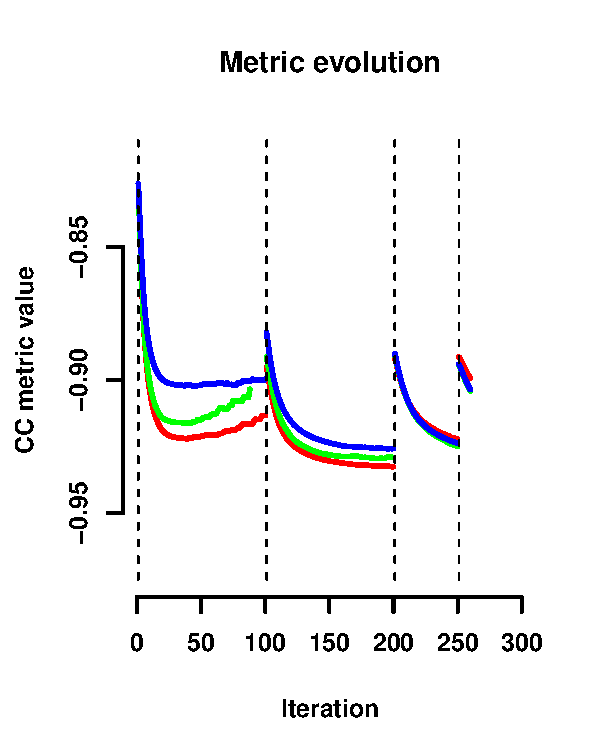
\includegraphics[width=67mm]{../WBIRStudy/SyNMetricEvolution.pdf} &
  \hspace{-15mm}
  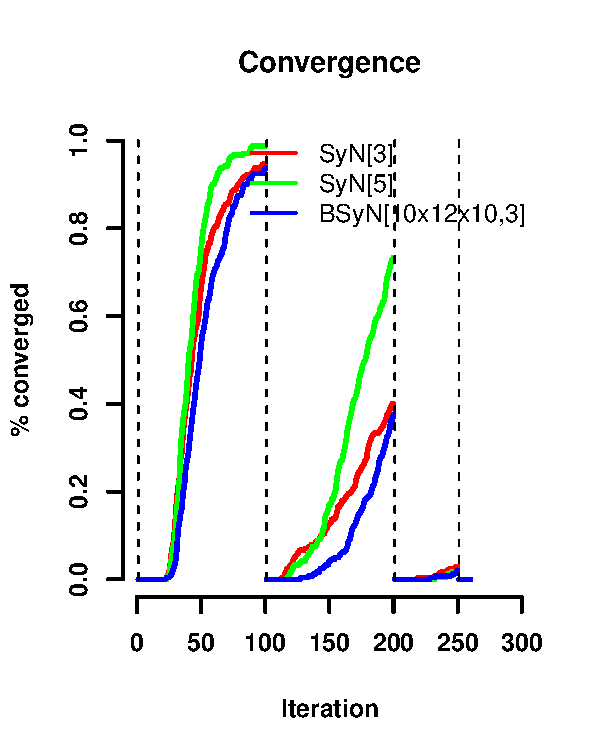
\includegraphics[width=67mm]{../WBIRStudy/SyNConvergences.pdf}
\end{tabular}
\end{center}

\end{frame}


%%%%%%%%%%%%%%%%%%%%%%%%%%%%%
%%  Closing slide
%%%%%%%%%%%%%%%%%%%%%%%%%%%%%

\begin{frame}{Thank you}
  \begin{center}
  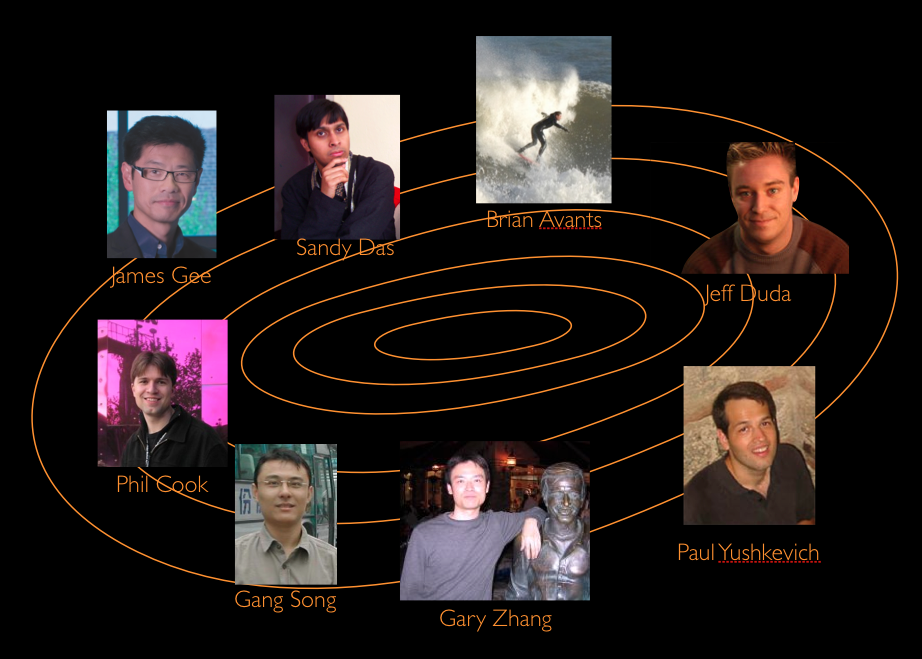
\includegraphics[height=6cm]{PICSL.png} \\
  and the \sout{users} co-developers.
  \end{center}
\end{frame}


%\begin{frame}
%\frametitle{Rigid body dynamics}
%
%\tikzstyle{na} = [baseline=-.5ex]
%
%\begin{itemize}[<+-| alert@+>]
%    \item Coriolis acceleration
%        \tikz[na] \node[coordinate] (n1) {};
%\end{itemize}
%
%% Below we mix an ordinary equation with TikZ nodes. Note that we have to
%% adjust the baseline of the nodes to get proper alignment with the rest of
%% the equation.
%\begin{equation*}
%\vec{a}_p = \vec{a}_o+\frac{{}^bd^2}{dt^2}\vec{r} +
%        \tikz[baseline]{
%            \node[fill=blue!20,anchor=base] (t1)
%            {$ 2\vec{\omega}_{ib}\times\frac{{}^bd}{dt}\vec{r}$};
%        } +
%        \tikz[baseline]{
%            \node[fill=red!20, ellipse,anchor=base] (t2)
%            {$\vec{\alpha}_{ib}\times\vec{r}$};
%        } +
%        \tikz[baseline]{
%            \node[fill=green!20,anchor=base] (t3)
%            {$\vec{\omega}_{ib}\times(\vec{\omega}_{ib}\times\vec{r})$};
%        }
%\end{equation*}
%
%\begin{itemize}[<+-| alert@+>]
%    \item Transversal acceleration
%        \tikz[na]\node [coordinate] (n2) {};
%    \item Centripetal acceleration
%        \tikz[na]\node [coordinate] (n3) {};
%\end{itemize}
%
%% Now it's time to draw some edges between the global nodes. Note that we
%% have to apply the 'overlay' style.
%\begin{tikzpicture}[overlay]
%        \path[->]<1-> (n1) edge [bend left] (t1);
%        \path[->]<2-> (n2) edge [out=10, in=-100] (t2);
%        \path[->]<3-> (n3) edge [out=10, in=-100] (t3);
%\end{tikzpicture}
%\end{frame}





%\begin{frame}{A bit of history\ldots}
%\end{frame}
%
%\begin{frame}{Examples}
%\begin{block}{Ein Beispiel mit der Umgebung \texttt{block}}
%Es ist offensichtlich, dass wir hier zwei Logos auf der Folie haben.
%\end{block}
%
%\end{frame}
%
%
%\begin{frame}
%     \begin{columns}[t] % contents are top vertically aligned
%     \begin{column}[T]{5cm} % each column can also be its own environment
%     Contents of first column \\ split into two lines
%     \end{column}
%     \begin{column}[T]{5cm} % alternative top-align that's better for graphics
%          
\includegraphics[height=3cm]{pengbrew.png}
%     \end{column}
%     \end{columns}
%\end{frame}
%
%\begin{frame}
%        \frametitle{`Hidden higher-order concepts?'}
%        \begin{itemize}[<+->]
%        \item The truths of arithmetic which are independent of PA in some 
%        sense themselves `{contain} essentially {\color{blue}{hidden higher-order}},
%         or infinitary, concepts'???
%        \item `Truths in the language of arithmetic which \ldots
%        \item   That suggests stronger version of Isaacson's thesis. 
%        \end{itemize}
%\end{frame}


%\section[Outline]{Shit}
%\frame{\tableofcontents}
%
%\section{Introduction}
%
%\frame {
%	\frametitle{First Frame}
%	\begin{itemize}
%		\item<1->One good argument
%		\item<2->Another good argument, after one click
%		\item<3->Last one, after another click
%	\end{itemize}
%}
%
%\section{Next Section}
%
%\subsection{First Sub Section}
%
%\frame {
%	\frametitle{Second Frame}
%	This text will stay on all pages.
%	\only<1>{
%		\begin{itemize}
%			\item<1->This will only appear on the first page
%			\item<1->This is also only for the first page
%		\end{itemize}
%	}
%	\only<2>{
%		\begin{itemize}
%			\item<2->This will only appear on the second page
%		\item<2->This is also only for the second page
%		\end{itemize}
%      }
%}
%
%\subsection{Second Sub Section}
%
%\frame {
%	\frametitle{Last Frame}
%	This is the last frame
%}

\end{document}